\documentclass[a4paper,11pt]{article}
\usepackage{assignment_style}
\usetikzlibrary{patterns}
\newcounter{problem}
\newenvironment{problem}[1][]{%
	\refstepcounter{problem}\par \medskip
	\noindent \textbf{Problem~\theproblem.#1 \rmfamily}{\medskip}
}

\newenvironment{solution}{ \noindent \textbf{Solution: \medskip}}{}
% To make solutions not visible use the command \excludecomment{solution} %
%\excludecomment{solution}

\title{Assignment 1 \\ \vspace{2em} \large WSU Economics PhD Math Bootcamp }
\date{}
\begin{document}
\maketitle

\begin{problem}
%Leon application page 23-25
Consider an economy with three sectors: farming, manufacturing and textiles.
Each sector produces its goods and then trades (through barter) with the other sectors.
Hence the three kinds of goods move between sectors.
Let the following table describe the results of trade.

\vspace{1em}
\begin{center}
\begin{tabular}{ c | c c c }\hline\hline
	& F & M & T \\ \hline
F & $\frac{1}{2}$ & $\frac{1}{3}$ & $\frac{1}{2}$ \\
M & $\frac{1}{4}$ & $\frac{1}{3}$ & $\frac{1}{4}$ \\
T & $\frac{1}{4}$ & $\frac{1}{3}$ & $\frac{1}{4}$ \\
\hline
\end{tabular}
\end{center}
The table is interpreted is as follows.  Let $x_1$ be the total value of farm goods, $x_2$ the total value of manufacturing goods and $x_3$ the total value of textile goods.
The first column of the table describes where the farming sectors output goes -- $1/2$ to themselves, $1/4$ to manufacturing and $1/4$ to textiles.
The first row describes the value of the farming sectors inputs -- $1/2$ from farming itself, $1/3$ manufacturing goods and $1/2$.
Hence the total value of farm goods is $x_1 = (1/2)x_1 + (1/3)x_2 + (1/2)x_3$.
Doing the same for the other sectors gives the system
\begin{align}
	x_1 &= \frac{1}{2}x_1 + \frac{1}{3}x_2 + \frac{1}{2}x_3 \nonumber \\
	x_2 &= \frac{1}{4}x_1 + \frac{1}{3}x_2 + \frac{1}{4}x_3 \nonumber \\
	x_3 &= \frac{1}{4}x_1 + \frac{1}{3}x_2 + \frac{1}{4}x_3 \nonumber
\end{align}

Turn the above system into a homogenous system and then solve the system to determine the total values of goods $x_1,x_2,x_3$.
\end{problem}
\insblock{Problem 1 Note}{Understand the definition of a homogenous system of linear equations and apply the appropriate matrix manipulations to solve the system.}
\begin{solution}
The reduced row echelon form for the augmented system is
\begin{align}
\left[
	\begin{matrix}
		1 & 0 & -\frac{5}{3} & | 0 \nonumber \\
		0 & 1 & -1 & | 0 \nonumber \\
		0 & 0 & 0 & | 0 \nonumber
	\end{matrix}
\right]
\end{align}
There is one free variable, $x_3$.
If we let $x_3=3$ then the solution is $(5,3,3)$.
\end{solution}

\begin{problem}
%Leon section 1.2 Problem 5 part (g)
	Determine whether the following system is inconsistent.  If not inconsistent and no free variables, find the unique solution.  If there are free variables find all solutions (describe the set).
	\begin{align}
		x_1 + x_2 + x_3 + x_4 &= 0 \nonumber \\
		2x_1 + 3x_2 -x_3 -x_4 &= 2 \nonumber \\
		3x_1 + 2x_2 + x_3 + x_4 &= 5 \nonumber \\
		3x_1 + 6x_2 -x_3 - x_4 &= 4 \nonumber
	\end{align}
\end{problem}
\insblock{Problem 2 Note}{This problem tests the idea that any linear system as either no solutions, 1 solution or an infinite number of solutions and you need to apply the appropriate methods to determine the case for the above system and how to describe the solution. The following problem tests the same concepts.}
\begin{solution}
	The system is inconsistent
\end{solution}

\begin{problem}
%Leon section 1.2 Problem 5 part (i)
	Determine whether the following system is inconsistent.  If not inconsistent and no free variables, find the unique solution.  If there are free variables find all solutions (describe the set).
	\begin{align}
		-x_1 + 2x_2 -x_3 &= 2 \nonumber \\
		-2x_1 + 2x_2 + x_3 &= 4 \nonumber \\
		3x_1 + 2x_2 + 2x_3 &= 5 \nonumber \\
		-3x_1 + 8x_2 + 5x_3 &= 17 \nonumber
	\end{align}
\end{problem}
\begin{solution}
	The system is consistent with no free variables and the unique solution is $(0, 3/2, 1)$.
\end{solution}

\begin{problem}

	Find the inverse matrix for the following matrices:
\[
	(\text{a}) \; \left[\begin{matrix}
		-1 & 1 \\
		1 & 0
	\end{matrix}\right] \qquad
	(\text{b}) \; \left[\begin{matrix}
		2 & 5 \\
		1 & 3
	\end{matrix}\right] \qquad 
	(\text{c}) \; \left[\begin{matrix}
		2 & 6 \\
		3 & 8
	\end{matrix}\right] \qquad
	(\text{d}) \; \left[\begin{matrix}
		1 & 1 & 1 \\
		0 & 1 & 1 \\
		0 & 0 & 1		
	\end{matrix}\right] \qquad
\]
\[
	(\text{e}) \; \left[\begin{matrix}
		2 & 0 & 5 \\
		0 & 3 & 0 \\
		1 & 0 & 3		
	\end{matrix}\right] \qquad
	(\text{f}) \; \left[\begin{matrix}
		-1 & -3 & -3 \\
		2 & 6 & 1 \\
		3 & 8 & 3 		
	\end{matrix}\right] \qquad
	(\text{g}) \; \left[\begin{matrix}
		1 & 0 & 1 \\
		-1 & 1 & 1 \\
		-1 & -2 & -3
	\end{matrix}\right]
\]
\end{problem}
\insblock{Problem 4 Note}{Tests understanding of the definition of an inverse matrix and how to calculate it for $2\times 2$ and $3\times 3$ systems.}
\begin{solution}
\[
	(\text{a}) \; \left[\begin{matrix}
		0 & 1 \\
		1 & 1
	\end{matrix}\right] \qquad
	(\text{b}) \; \left[\begin{matrix}
		3 & -5 \\
		-1 & 2
	\end{matrix}\right] \qquad
	(\text{c}) \; \left[\begin{matrix}
		-4 & 3 \\
		3/2 & -1
	\end{matrix}\right] \qquad
	(\text{d}) \; \left[\begin{matrix}
		1 & -1 & 0 \\
		0 & 1 & -1 \\
		0 & 0 & 1
	\end{matrix}\right] \qquad
\]
\[
	(\text{e}) \; \left[\begin{matrix}
		3 & 0 & -5 \\
		0 & 1/3 & 0 \\
		-1 & 0 & 2
	\end{matrix}\right] \qquad
	(\text{f}) \; \left[\begin{matrix}
		2 & -3 & 3 \\
		-3/5 & 6/5 & -1 \\
		-2/5 & -1/5 & 0
	\end{matrix}\right] \qquad
	(\text{g}) \; \left[\begin{matrix}
		-1/2 & -1 & -1/2 \\
		-2 & -1 & -1 \\
		3/2 & 1 & 1/2
	\end{matrix}\right] \qquad
\]
\end{solution}

\begin{problem}
%Leon section 2.1 problem 3 (d),(g)
Evaluate the following determinants
\[
	(\text{a}) \; \left|\begin{matrix}
		4 & 3 & 0 \\
		3 & 1 & 2 \\
		5 & -1 & -4		
	\end{matrix}\right| \qquad
	(\text{b}) \; \left|\begin{matrix}
		2 & 0 & 0 & 1 \\
		0 & 1 & 0 & 0 \\
		1 & 6 & 2 & 0 \\
		1 & 1 & -2 & 3
	\end{matrix}\right|
\]
\end{problem}
\insblock{Problem 5 Note}{Tests the ability to calculate the determinant of a linear system.}
\begin{solution}
	(a) 58; \; (b) 8
\end{solution}

\begin{problem}
%Leon Section 2.3 Cramer's rule example page 107
Use Cramer's rule to solve the following system
\begin{align}
	x_1 + 2x_2 + x_3 &=5 \nonumber \\
	2x_1 + 2x_2 + x_3 &= 6 \nonumber \\
	x_1 + 2x_2 + 3x_3 &= 9 \nonumber
\end{align}
\end{problem}
\begin{solution}
\[
	x_1 = \frac{-4}{-4} = 1, \qquad x_2 = \frac{-4}{-4} = 1, \qquad x_3 = \frac{-8}{-4} = 2
\]
\end{solution}

\begin{problem}
Let $A$ and $B$ be $6\times 6$ matrices, with $\det(A) = -10$ and $\det(B) = 5$.
Use the properties of determinants to compute
\begin{enumerate}[(a)]
	\item $\det(3A)$
	\item $\det(A^{T} B^{-1})$
\end{enumerate}

\end{problem}
\insblock{Problem 7 Note}{Tests understanding of the properties of determinants as they apply to matrix algebra.}
\begin{solution}
\begin{enumerate}[(a)]
	\item $\det(3A) = 3^6 \det(A) = 729(-10) = -7290$.
	\item \begin{align}
				\det(A^T B^{-1}) &= \det(A^T) \cdot \det(B^{-1}) \nonumber \\
				&= \left( \det(A) \right) \frac{1}{\det(B)} \nonumber \\
				&= -10 \frac{1}{5} \nonumber \\
				&= -2 \nonumber
		  \end{align}
\end{enumerate}
\end{solution}

\begin{problem}
Prove that if $A$ is invertible, then $\det(A^{-1}) = \frac{1}{\det(A)}$
\end{problem}
\insblock{Problem 8 Note}{Tests understanding of properties of determinants and inverses as well as the idea of mathematical proof.}
\begin{solution}
	By multiplicative properties of the determinant
	\[
		\det(AA^{-1}) = \det(A) \cdot \det(A^{-1})
	\]
	We also know that $AA^{-1} = I_n$, the $n\times n$ identity matrix, and $\det(I_n) = 1$ (this can be seen because $I_n$ is a diagonal matrix).
	So we have
	\[
		\det(A)\cdot \det(A^{-1}) = 1
	\]
	Solving for $\det(A)$, we get $\det(A^{-1}) = \frac{1}{\det(A)}$ where is it okay to divide by $\det(A)$ because we know that $\det(A) \neq 0$ because $A$ is invertible. \qedsymbol
\end{solution}

\begin{problem}
Let $A$ be a $3\times 3$ matrix with $\det(A) = 5$.
Find each of the following if possible.
\begin{enumerate}[(a)]
	\item $\det(A^T)$
	\item $\det(A + I)$
	\item $\det(2A)$.
\end{enumerate}
\end{problem}
\insblock{Problem 9 Note}{Tests understanding of matrix algebra and its effects on the value of a determinant of a linear system.  Also, remember that one reason we care about determinants is because they can often tell us something about the solution space to a linear system.}
\begin{solution}
\begin{enumerate}[(a)]
	\item $\det(A^T) = \det(A) = 5$
	\item There is not enough information
	\item $\det(2A) = 2^3 \det(A) = 40$.
\end{enumerate}
\end{solution}

\begin{problem}
	What are the dimensions of the following subsets of $\mathbb{R}^3$?
	\begin{enumerate}[(i)]
		\item The origin?
		\item A line through the origin?
		\item A plane which passes through the origin?
	\end{enumerate}
\end{problem}
\insblock{Note}{Tests understanding of the idea of linear spaces and their dimension -- Hint: linear spaces are the \textit{span} of a set of \textit{basis vectors}.}
\begin{solution}
	\begin{enumerate}[(i)]
		\item The origin has dimension zero.  Note that $\alpha(0,0,0) = (0,0,0)$ is true for all $\alpha \in \mathbb{R}$ so its always linearly dependent.
		\item A line through the origin has dimension 1.
		\item A plane has dimension 2.
	\end{enumerate}
\end{solution}


\begin{problem}
%Duke Mathcamp notes problem 1.23 and 1.24
	For $\mathbf{a},\mathbf{x} \in \mathbb{R}^n$, consider the equation $\mathbf{a} \cdot \mathbf{x} = 0$ and its solution set $X(\mathbf{a}) = \{ \mathbf{x} \in \mathbb{R}^n \; | \; \mathbf{a} \cdot \mathbf{x} = 0 \}$.  
	\begin{enumerate}[(i)]
		\item Show that $X(\mathbf{a})$ is a linear subspace.
		\item Show the dimension of $X(\mathbf{a})$.
	\end{enumerate}
\end{problem}
\insblock{Problem 11 Note}{Tests understanding of \textit{null spaces} of linear functions (matrices).  Null spaces can often represent the space of solutions to an economic problem.  It also tests your understanding of a linear subspace and how to show a set is one as well as identify its dimension.}
\begin{solution}
	\begin{enumerate}[(i)]
		\item If $x,x' \in X(a)$ then $a\cdot x = a\cdot x' = 0$.
		Hence $a\cdot x + a\cdot x' = a\cdot(x + x') = 0$ and this implies that $x+x' \in X(a)$.
		Again let $x \in X(a)$ then $a\cdot x = 0$ and $\alpha a\cdot x = 0$ as well.
		Moving the constant we see that $a \cdot (\alpha x) = 0$ which means that $\alpha x \in X(a)$.
		\item Clearly the dimension of $\mathbb{R}^n$ is $n$.
		The vector $a$ represents a linear mapping with one row.
		The linear span of $a$ is contained in a subspace with dimension 1.
		The set $X(a)$ contains all the vectors which are orthogonal to $a$.
		By the rank nullity theorem we know that $\text{rank}(f) + Null(f) = dim(\mathbb{R}^n)$.
		Hence the dimension of the null space $X(a)$ is $dim(\mathbb{R}^n) - \text{rank}(f) = n - 1$.
		
		Another way to look at this is by using what you found in Problem 1 and recognizing that $X(a)$ is a hyperplane in $\mathbb{R}^n$ passing through the origin.
		In Problem 1, you found that a plane in $\mathbb{R}^3$ passing through the origin had dimension $3-1 = 2$.
		Well a hyperplane is just a plane, so if $X(a)$ is a hyperplane through the origin in $\mathbb{R}^n$ it must have dimension $n-1$.
	\end{enumerate}
\end{solution}

\paragraph{Some Definitions}
The following definitions describe the ``greater than or equal to'' type of ordering on $\mathbb{R}^n$ that will be important for answering Problem 3.
\begin{definition}
	Let $\mathbf{x}$ and $\mathbf{y}$ be vectors in $\mathbb{R}^n$.  We define the following relations:
	\begin{itemize}
		\item $\mathbf{x} = \mathbf{y}$ iff $x_i = y_i$ for all $i=1,2,\dots, n$.
		\item $\mathbf{x} \geq \mathbf{y}$ iff $x_i \geq y_i$ for all $i=1,2,\dots, n$.
		\item $\mathbf{x} > \mathbf{y}$ iff $x_i \geq y_i$ and $x\neq y$ -- meaning there is at least one element $j$ such that $x_j > y_j$.
		\item $\mathbf{x} \gg \mathbf{y}$ iff $x_i > y_i$ for all $i=1,2,\dots, n$.
	\end{itemize}
\end{definition}

\begin{problem}
	Suppose $\mathbf{a},\mathbf{x},\mathbf{y} \in \mathbb{R}^n$ and $\mathbf{a}\cdot \mathbf{x} > \mathbf{a} \cdot \mathbf{y}$.  Does it follow that $x > y$? [Hint: do not divide both sides by $\mathbf{a}$]
\end{problem}
\insblock{Problem 12 Notes}{Tests understanding of linear functions (functionals in particular) and how they can \textit{order} the vectors in a linear subspace.  It also introduces and provides practice with vector orderings that come up relatively frequently.  Also note that the linear function created by $\mathbf{a}\cdot \mathbf{x}$ for $\mathbf{x}\in X$ two \textit{half-spaces} are created that order some vectors ``above'' others.}
\begin{solution}\\
	Let $\mathbf{a},\mathbf{x},\mathbf{y} \in \mathbb{R}^n$ (note these are vectors) and let $\mathbf{a} \cdot \mathbf{x} > \mathbf{a} \cdot \mathbf{y}$.
	Note that both $\mathbf{a}\cdot \mathbf{x}$ and $\mathbf{a}\cdot \mathbf{y}$ are real numbers so the $>$ here refers to the ordering on the real line, while the comparison we want to investigate $\mathbf{x} > \mathbf{y}$ is an ordering on vectors (as defined before the problem).
	Lets consider the value $r_y = \mathbf{a} \cdot \mathbf{y}$.
	Consider the hyperplane $X(\mathbf{a},r_y) = \{ \mathbf{z} \in \mathbb{R}^n: \mathbf{a} \cdot \mathbf{z} = r_y \}$ and the ``upper'' half-space $X^+(\mathbf{a},r_y) = \{ \mathbf{z} \in \mathbb{R}^n: \mathbf{a} \cdot \mathbf{z} \geq r_y \}$.
	Now we know that $\mathbf{a}\cdot \mathbf{x} > r_y$ so we can be sure $\mathbf{x} \in X^+(\mathbf{a},r_y)$.
	Let $Y = \{ \mathbf{z} \in \mathbb{R}^n: z_i \geq y_i \; \forall i = 1, \dots, n\}$ be the set of all vectors $\mathbf{z}$ such that $\mathbf{z} \geq \mathbf{y}$.
	When $Y \subsetneq X^+(\mathbf{a},r_y)$ then its possible for $\mathbf{a}\cdot \mathbf{x} > \mathbf{a}\cdot \mathbf{y}$ and yet $\neg (\mathbf{x} > \mathbf{y})$.
	Consider the two-dimensional graph below.
	Each of the points $\mathbf{x},\mathbf{x}',\mathbf{x}''$ are contained in $X^+(\mathbf{a},r_y)$ yet are not in $Y$.
	So its possible for $\mathbf{a}\cdot \mathbf{x} > \mathbf{a}\cdot \mathbf{y}$ and yet $\mathbf{x} \leq \mathbf{y}$.
	
	\begin{figure}[htbp]
	\centering
	\caption{Hyperplanes, Half-spaces and Vector Ordering}
	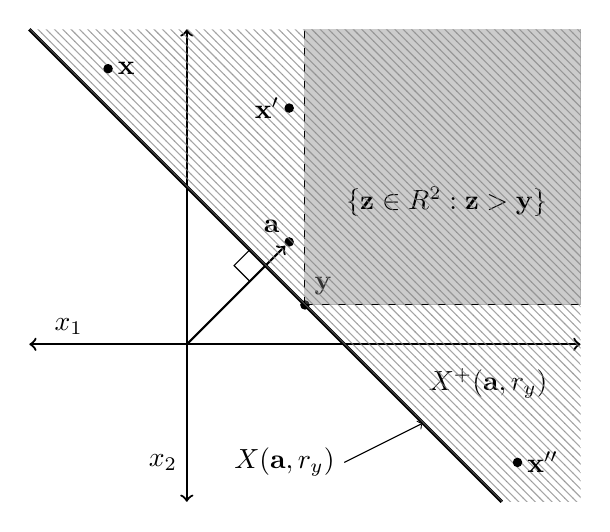
\begin{tikzpicture}
		\draw[<->, thick] (0,4) -- (0,-2);
		\draw[<->, thick] (5,0) -- (-2,0);
		\node[left] at (0,-1.5) {$x_2$};
		\node[above] at (-1.5,0) {$x_1$};
		\draw (1.3,1.3) node[anchor=south east] {$\mathbf{a}$};
		\draw[fill=black] (1.5,0.5) circle[radius=1.5pt];
		\draw (1.5,0.5) node[above right] {$\mathbf{y}$};
		\draw[fill=black] (1.3,1.3) circle[radius=1.5pt];
		\draw[arrows=->,thick] (0,0) -- (1.25,1.25);
		\draw[fill=gray, draw=gray, opacity=0.4] (1.5,4) -- (1.5,0.5) -- (5,0.5) -- (5,4);
		\draw[dashed, thin] (1.5,0.5) -- (1.5,4);
		\draw[dashed, thin] (1.5,0.5) -- (5,0.5);
		\node[above] at (3.3,1.5) {$\{ \mathbf{z} \in \mathbb{R}^2: \mathbf{z} > \mathbf{y}\}$};
		\draw[very thick] (-2,4) -- (1,1) -- (4,-2);
		\node[right] at (2.95,-0.5) {$X^+(\mathbf{a},r_y)$};
		\node[left] at (2,-1.5) {$X(\mathbf{a},r_y)$};
		\draw[->] (2,-1.5) -- (3,-1);
		\draw[pattern=north west lines, pattern color=gray, opacity=0.7,draw=none] (-2,4) -- (1,1) -- (4,-2) -- (5,-2) -- (5,4);
		\draw[fill=black] (-1,3.5) circle[radius=1.5pt] node[right] {$\mathbf{x}$};
		\draw[fill=black] (1.3,3) circle[radius=1.5pt] node[left] {$\mathbf{x}'$};
		\draw[fill=black] (4.2,-1.5) circle[radius=1.5pt] node[right] {$\mathbf{x}''$};
		\draw (0.8,1.2) -- (0.6,1) -- (0.8,0.8);
	\end{tikzpicture}	
	\end{figure}
 
	
\end{solution}

\begin{problem}
	Let $X$ be a vector space and consider a function $f:X \rightarrow \mathbb{R}$ defined for some $\mathbf{a} \in X$ defined as $f_a(\mathbf{x}) = \mathbf{a} \cdot \mathbf{x}$.
	\begin{enumerate}[(i)]
		\item Prove that $f_a(\mathbf{x}) = \mathbf{a}\cdot \mathbf{x}$ is a linear function.
		\item Let $X^* = \{ f:X \rightarrow R \; | \; f \text{ is linear}\}$ be the set of all linear functions from $X$ into $\mathbb{R}$.
		Prove that for all $f \in X^*$ there exists an $\mathbf{a}\in X$ such that $f(\mathbf{x}) = \mathbf{a} \cdot \mathbf{x}$.
		\item (\textbf{Optional}) Define function addition as $f+g = f(\mathbf{x})+g(\mathbf{x})$ and function scaling as $\alpha f = \alpha f(\mathbf{x})$ over the set $X^*$.  Prove or disprove the following statement: $X^*$ \textit{with the defined operations is a linear vector space}.
		\item (\textbf{Optional}) What is dimension of $X^*$?
	\end{enumerate}
\end{problem}
\insblock{Problem 13 Note}{Tests understanding of the definition of a linear function (mapping, transformation) and how to use it.  Tests understanding of linear functionals and how they can be represented by vectors and the (inner) dot product.  The optional parts are good practice in applying the axioms of abstract vector spaces and identifying dimension.}
\begin{solution} \textbf{and hints...}
	\begin{enumerate}[(i)]
		\item So for this problem just assume that $X = \mathbb{R}^n$.
Then $a\cdot x = a_1 x_1 + \cdots + a_n x_n$.
Given two vectors $x,y \in \mathbb{R}^n$ and scalars $\alpha, \beta \in \mathbb{R}$ we have
\begin{align}
	a \cdot (\alpha x + \beta y) &= a\cdot (\alpha x) + a\cdot (\beta y) \nonumber \\
	&= \alpha(a\cdot x) + \beta (a\cdot y) \nonumber 
\end{align}
therefore its a linear map.
	\item For part (ii), this is basically the proof that linear transformations between real vector spaces can be represented by real valued matrices.
In this case the matrices will all be $n\times 1$.
Consider a function $f\in X^*$.
By definition $f$ is a linear map from $X = \mathbb{R}^n$ to $\mathbb{R}$.
Because $X$ is a linear subspace and $\mathbb{R}$ is a linear subspace and $f$ is a linear map we know that $f(X)$ is a linear subspace in $\mathbb{R}$.
Because $X$ and $f(X)$ are subspaces they have a basis.
Let $(\mathbf{e}_1,\dots, \mathbf{e}_n)$ be the coordinate vectors for $\mathbb{R}^n$ (which are a basis for $X$).
Then for any $x\in X$ we can write $\mathbf{x} = x_1 \mathbf{e}_1 + \cdots + x_n \mathbf{e}_n$ (a linear combination of the basis vectors).
Applying our function $f$ to $x$ gives us
\begin{align}
	f(\mathbf{x}) &= f( x_1 \mathbf{e}_1 + \cdots + x_n \mathbf{e}_n ) \nonumber \\
	&= x_1 f(\mathbf{e}_1) + \cdots + x_n f(\mathbf{e}_n) \nonumber
\end{align}
Since $\mathbf{e}_i$, for $i=1,\dots,n$ is a vector we know $f(\mathbf{e}_i) \in \mathbb{R}$.
For all $i = 1,\dots, n$ define $f(\mathbf{e}_i) = a_i$.
Then 
\begin{align}
	f(\mathbf{x}) &= x_1 a_1 + \cdots + x_n a_n \nonumber \\
	&= a_1 x_n + \cdots + a_n x_n \nonumber \\
	&= \mathbf{a} \cdot \mathbf{x} \nonumber
\end{align}
so we can define the $\mathbf{a} = (f(\mathbf{e}_1), \dots, f(\mathbf{e}_n))$.
	\item For part (iii), you should use the defined operations to show that the vector space axioms hold for this set so that its a vector space.
The key operations are that if $f$ and $g$ are linear functions in the set, then these will be our vectors.
So $f + g$ is defined as $f(x) + g(x)$ where $x$ is a vector in $X$.
If $\alpha$ is a real number, then we scale the vectors in $X^*$ as $\alpha f = \alpha f(x)$.

Let $\mathbf{u},\mathbf{v},\mathbf{w} \in V$  where $V$ is a vector space.
Let $c,d \in \mathbb{R}$.
Then the following are the axioms of an abstract vector space.
	\begin{enumerate}[1.]
		\item $\mathbf{u} + \mathbf{v} \in V$
		\item $\mathbf{u} + \mathbf{v} = \mathbf{v} + \mathbf{u}$
		\item $(\mathbf{u} + \mathbf{v}) + \mathbf{w} = \mathbf{u} + (\mathbf{v} + \mathbf{w})$
		\item $\exists \mathbf{0} \in V$ such that $\forall \mathbf{u} \in V, \; \mathbf{u} + \mathbf{0} = \mathbf{u}$
		\item $\forall \mathbf{u} \in V, \; \exists -\mathbf{u} \in V$ such that $\mathbf{u} + (-\mathbf{u}) = \mathbf{0}$
		\item $\forall c \in \mathbb{R}$, $c\mathbf{u} \in V$.
		\item $c(\mathbf{u} + \mathbf{v}) = c \mathbf{u} + c \mathbf{v}$
		\item $(c+d)\mathbf{u} = c\mathbf{u} + d \mathbf{v}$
		\item $(cd)\mathbf{u} = c(d\mathbf{u})$
		\item $1\mathbf{u} = \mathbf{u}$
	\end{enumerate}
All the axioms should be tested.
	\item For part (iv) the idea is to use what we just learned in part (ii), that every linear functional $f \in X^*$ can be uniquely determined by a vector $\mathbf{a} = (f(\mathbf{e}_1),\dots,f(\mathbf{e}_n))$.
We can think about finding a set of such $\mathbf{a}$ vectors.
For example suppose we have a set of $n$ vectors, say the coordinate vectors again, $(\mathbf{e}_1,\dots, \mathbf{e}_n)$, do each of these represent their own linear functional? Yes.
Now that we are calling them functionals, lets represent the set now as $\{f_1,\dots, f_n\}$.
At this point we establish that any linear functional is just a linear combination of these $n$ linear functionals and that the set is linearly independent.
Once you've done that you will have shown that a set of $n$ vectors is a basis for $X^*$ and therefore $\dim\left(X^*\right) = n$.
	\end{enumerate}
\end{solution}

\begin{problem}
	Prove that the set $Z$ is a subspace of $\mathbb{R}^3$.
	\[
		Z = \left\{ [x_1,x_2,x_3] \; | \; 4x_1 - x_2 + 5x_3 = 0 \right\}
	\]
\end{problem}
\insblock{Problem 14 Note}{Tests application of the definition of subspaces.}
\begin{solution}
	Let $a = [4,-1,5]$ and note that the equation in the definition of $Z$ is $4x_1 - x_2 + 5x_3 = a \cdot x$.  
	Hence we have the linear function $L(x) = a\cdot x$ and $a\cdot x = 0$ represents a homogenous system of equations.
	The set $Z$ represents the set of solutions $\{x \in \mathbb{R}^3 | a\cdot x = 0\}$ which is also the null space of the linear function $L(x) = a\cdot x$.
	The null space of any linear function is a subspace. \qedsymbol
\end{solution}


\begin{problem}
%Leon Ch 4 Section 1 # 17
Determine the null space and range of each of the following linear operators on $\mathbb{R}^3$.
\begin{enumerate}[(i)]
	\item $L(\mathbf{x}) = (x_3,x_2,x_1)^T$
	\item $L(\mathbf{x}) = (x_1,x_1,x_1)^T$
\end{enumerate}
\end{problem}
\insblock{Problem 15 Note}{Tests understanding of the definition and concept of null space (kernal) and range (column space) of a linear operator (matrix).}
\begin{solution}
	\begin{enumerate}[(i)]
		\item $Null(L) = \{\mathbf{0}\}$ and $L(\mathbb{R}^3) = \mathbb{R}^3$.
		\item $Null(L) = \text{Span}(\mathbf{e}_2,\mathbf{e}_3)$ and $L(\mathbb{R}^3) = \text{Span}(\mathbf{e}_1)$.
	\end{enumerate}
\end{solution}

\begin{definition}
	Let $X$ be a vector space and let $a \in X$ and $b \in \mathbb{R}$.
	A \textbf{hyperplane} in $X$ is a set of the form $H_a(b) = \{ x \in X: a\cdot x = b\}$ and associated with hyperplane $X$ are two \textbf{half-spaces} $H_a^{\geq}(b) = \{x\in X: a\cdot x \geq b \}$ and $H_a^{\leq}(b) = \{x\in X: a\cdot x \leq b\}$.
\end{definition}

\begin{problem}
	(\textbf{Optional}) What are the range of angles between vectors in $x \in H_a^{\leq}(0)$ and the vector $a$? What are the ranges of the angles between vectors $x\in H_a^{\geq}(0)$ and the vector $a$?
\end{problem}
\insblock{Problem 16 Note}{Tests knowledge and understanding of the Cauchy-Schwartz inequality, the dot product and their relationship to the angle between two vectors in a vector space.  It connects this concept to that of half-spaces.}
\begin{solution}
	For $H_a^{\geq}(0)$ the range on the angles between vectors $x$ and the vector $a$ are $\theta = [0,90]\cup [270,360]$ and the range on the angles between vectors $x$ in $H_a^{\leq}(0)$ and $a$ are $\theta = [90,270]$.
\end{solution}

\begin{problem}
%Simon & Blume exercise 27.19
	Which of the following are \emph{subspaces} of the vector space $M_{2,2}$ of $2\times 2$ matrices? Justify your answer.
	\begin{enumerate}[(i)]
		\item the set of $2\times 2$ real symmetric matrices.
		\item the set of $2\times 2$ real diagonal matrices.
		\item the set of $2\times 2$ real ``singular'' matrices (remember $M$ is singular if $det(M) = 0$).
		\item the zero matrix.
		\item the set of all $2\times 2$ nonsingular matrices
	\end{enumerate}
\end{problem}
\insblock{Problem 17 Note}{More practice applying definition of subspaces to spaces of specific matrices to show which are subspaces.}
\begin{solution}
	\begin{enumerate}[(i)]
		\item \begin{align}
			\alpha \left[\begin{matrix}
				a_{11} & a_{12} \\
				a_{12} & a_{22}
			\end{matrix}\right] +
			\beta \left[\begin{matrix}
				b_{11} & b_{12} \\
				b_{12} & b_{22}
			\end{matrix}\right] = 
			\left[\begin{matrix}
				\alpha a_{11} + \beta b_{11} & \alpha a_{12} + \beta b_{12} \\
				\alpha a_{12} + \beta b_{12} & \alpha a_{22} + \beta b_{22} 
			\end{matrix}\right] \nonumber
		\end{align}
	\item \begin{align}
			\alpha \left[\begin{matrix}
				a_{11} & 0 \\
				0 & a_{22}
			\end{matrix}\right] +
			\beta \left[\begin{matrix}
				b_{11} & 0 \\
				0 & b_{22}
			\end{matrix}\right] = 
			\left[\begin{matrix}
				\alpha a_{11} + \beta b_{11} & 0 \\
				0 & \alpha a_{22} + \beta b_{22} 
			\end{matrix}\right] \nonumber
		\end{align}
		\item This space is not a subspace.
		Consider the matrices 
		\[
			A = \left[\begin{matrix}
				1 & 0 \\
				0 & 0
			\end{matrix}\right] \qquad
			B = \left[\begin{matrix}
				0 & 0 \\
				0 & 1
			\end{matrix}\right]
		\]
		The $\det A = 0$ and $\det B = 0$, but $\det(A + B) = \det(I) = 1 \neq 0$.
		\item Yes it is a subspace as any linear combination of it is the zero matrix.
		\item Note that $\det I = 1 \neq 0$ and $\det(-I) = (-1)^2 \det I = 1 \neq 0$ but $I + (-I) = 0$ and the zero matrix is not invertible.
	\end{enumerate}
\end{solution}

\begin{problem}
	Let $f:\mathbb{R}^n \rightarrow \mathbb{R}^m$ be a linear function such that for all $y \in \mathbb{R}^m$ the set $\{x \in \mathbb{R}^n : f(x)=y\}$ is a singleton.
	\begin{enumerate}[(i)]
		\item Is the linear function $f$ invertible?
		\item If $f$ can be represented by matrix $A$, then show $A$ is invertible if and only if $\text{rank}(A) = m = n$.
		\item Suppose that an $n\times n$ matrix $A$ is invertible.  Does it follow that $[Ax = 0] \implies [x = 0]$?
		\item Suppose that $A$ is an $n \times n$ matrix and that $[Ax=0]\implies [x=0]$.
		Does it follow that $A$ is invertible?
	\end{enumerate}
\end{problem}
\insblock{Problem 18 Note}{Tests understanding of the requirements for the existence of an inverse function and its relationship to matrix inverses in the case of linear functions.  These concepts are then tied to some fundamental properties about the existence and uniqueness of the solution to a system of linear equations.}
\begin{solution}
\begin{enumerate}[(i)]
	\item Yes, the function is a bijection and so the inverse correspondence will be a function.
	\item ($\Leftarrow$) Suppose that $\text{rank}(A)=m=n$ and assume to the contrary that $A$ is not invertible.
	Then there must exist $y,x,x' \in \mathbb{R}^n$ with $x\neq x'$ such that $y=Ax=Ax'$.
	But this means that $A(x-x')=0$ with $(x-x')\neq 0$ and thus the columns of $A$ are linearly dependent. This means there can be, at most, $n-1$ linearly independent columns making the rank of $A$ less than $n$ - which is a contradiction.
	
	($\Rightarrow$) For the other direction, we can use proof by contrapositive.
	So assume $\text{rank}(A) \neq n$ and attempt to show that this implies $A$ is not invertible.
	Since $\text{rank}(A) \leq \dim \mathbb{R}^n = n$ we know $\text{rank}(A) < n$.
	Which means that the number of linearly independent columns of $A$ is less than $n$.
	Let $\mathbf{a}_1, \dots, \mathbf{a}_n$ represent the $n$ columns of $A$.
	Then $\exists \boldsymbol{\alpha} = (\alpha_1, \dots, \alpha_n) \neq \mathbf{0}$ such that $\alpha_1 \mathbf{a}_1 + \cdots + \alpha_n \mathbf{a}_n = \mathbf{0}$ which is equivalent $A \boldsymbol{\alpha} = \mathbf{0}$ so $Null(A)$ contains more elements than just the zero vector $\mathbf{0}$.
	Since multiple elements are mapped to the same vector, the function $f$ represented by $A$ is not injective and therefore not bijective and thus not invertible. \qedsymbol
	\item Let $A$ be invertible and for some vector $\mathbf{x}$ suppose $A\mathbf{x} = \mathbf{0}$.
	Then
	\begin{align}
		A\mathbf{x} &= \mathbf{0} \nonumber \\
		A^{-1} A \mathbf{x} &= A^{-1} \mathbf{0} \nonumber \\
		I_{n} \mathbf{x} &= \mathbf{0} \nonumber \\
		\mathbf{x} &= \mathbf{0} \nonumber
	\end{align}
	which establishes the result. \qedsymbol
	\item Let $A$ be an $n\times n$ matrix such that $Null(A) = \{\mathbf{0}\}$.
	Let $\mathbf{u} \neq \mathbf{v}$ be two nonzero vectors.
	Suppose $A \mathbf{u} = A \mathbf{v}$ then $A \mathbf{u} - A \mathbf{v} = \mathbf{0}$ and finally $A(\mathbf{u} - \mathbf{v}) = \mathbf{0}$.
	But $(\mathbf{u}-\mathbf{v})\neq \mathbf{0}$ which is impossible since only $\mathbf{0}$ is in the null space of $A$.
	This contradiction implies that $A$ is injective.
	By the rank nullity theorem we have $\dim \mathbb{R}^n = \dim Null(A) + \dim \text{img}(A)$ and since $\dim Null(A) = 0$ we have $n = 0 + \dim \text{img}(A)$ which implies $\dim \text{img}(A) = n$.
	This means the image of $A$ ( or of $f$) fills all of $\mathbb{R}^n$ and $A$ is surjective.
	Because it is injective and surjective $A$ is invertible. \qedsymbol 
\end{enumerate}
\end{solution}

\begin{problem}
	Let $y\in \mathbb{R}^n$ be a \textbf{netput} vector where each element $y_i$ for $i=1,\dots, n$ is a commodity.
	If $y_i < 0$ then $y_i$ is an input into a production process.
	If $y_i > 0$ then $y_i$ is an output of the production process.
	Let $F:\mathbb{R}^n \rightarrow \mathbb{R}$ be a \emph{transformation function} and we define the set $Y =\{y\in \mathbb{R}^n : F(y) \leq 0 \}$ and we'll call $Y$ a technology.
	The technology $Y$ describes all the feasible production plans a firm can choose (i.e., combinations of feasible inputs and outputs).
	We will assume that $Y$ is a convex set.
	Now let $p\in \mathbb{R}^n$ where $p \gg 0$ be vector prices for the $n$ commodities in any bundle $y\in Y$.
	Note that for fixed $p$, we can define a function $T_p(y) = p\cdot y$ for all $y \in Y$.
	The function $T_p(y)$ represents the profit (revenue minus costs) of choosing production plan $y$ when input and output prices are given by $p$.
	Firms want to choose some feasible production plan $y^*$ that satisfies $T_p(y^*) = \max\{p\cdot y: y\in Y\}=\pi(p)$.
	\begin{enumerate}[(i)]
		\item If $\pi(p)$ is the maximum achievable profit for firms given technology $Y$ and prices $p$ the profit-maximizing production plans are $\{ y \in Y: p\cdot y = \pi(p) \}$. Now consider the set $\{y \in \mathbb{R}^n: p\cdot y = \pi(p)\}$. Is this a hyperplane?  If so, show that $Y$ is contained in one of the half-spaces of $p\cdot y = \pi(p)$ and specify which one (i.e., upper or lower).
		\item Does the set $\{y\in \mathbb{R}^n: p\cdot y = \pi(p)\}$ ``touch'' the technology $Y$? i.e, is it the case that
		\[
			\min_{y\in Y}\; | p\cdot y - \pi(p)| = 0
		\]
		If so, what does this say about the value of $F(y^*)$ for any $y^* \in \{y\in Y: p\cdot y = \pi(p)\}$?
		\item \textbf{Optional} (Duality) Consider the sets of the form $A(p) = \{ y \in \mathbb{R}^n : p\cdot y \leq \pi(p)\}$ and we create a collection of sets $\{ A(p) \subset \mathbb{R}^n : p \in \mathbb{R}^n\}$.
		Show that the following equality is true.
		\[
			Y = \bigcap_{p\in \mathbb{R}^n} A(p)
		\]
	\end{enumerate}
\end{problem}
\insblock{Problem 19 Note}{Application of key concepts you've been working on.  In particular the idea of the support function (which is a linear functional) and how it relates to the profit to the firm of a particular production plan.  This function creates half-spaces and the hyperplane can be tangent to a curve representing optimal points.  If this problem is difficult don't worry it is some of the more difficult concepts you'll see in the fall micro class.}
\begin{solution}
	See the hints I provided through email.
\end{solution}


\end{document}